\section{Riduzioni}
Una riduzione traduce un'istanza di un problema in un'istanza di un altro problema. \\
Poi usa la soluzione del secondo problema per risolvere il primo. \\
La traduzione deve essere:
\begin{itemize}
    \item Corretta: la risposta dell'istanza tradotta deve essere la stessa della risposta dell'istanza originale.
    \item Efficiente: la traduzione deve essere eseguita in tempo polinomiale e spazio logaritmico rispetto alla dimensione dell'input originale. \\
    In questo modo, se il secondo problema é risolvibile in tempo polinomiale, anche il primo lo é.
\end{itemize}

Formalmente: \\
Una riduzione é una funzione $R$ che traduce un'istanza $x$ di un problema $L_1$ in una istanza $R(x)$ di un problema $L_2$
preservando le risposte. \\

Un linguaggio $L_1$ é riducibile a un linguaggio $L_2$ se esiste una funzione $R$ calcolabile da una MdT deterministica:
\begin{itemize}
\item tale che per ogni stringa $x$, $x \in L_1 \iff R(x) \in L_2$;
\item calcolabile in tempo polinomiale rispetto alla lunghezza di $x$;
\item calcolabile in spazio logaritmico rispetto alla lunghezza di $x$.
\end{itemize}


\subsection{Riduzione di $\MAXFLOW$ a $\REACHABILITY$}
\label{riduzione:maxflow_reachability}

\subsubsection{Determinare se un flusso é ottimo}
Consideriamo un flusso qualsiasi $f$. Ci interessa sapere se é ottimo oppure no. \\
Supponiamo che $f$ non é ottimo, allora esiste un flusso $f'$ con valore maggiore di $f$. \\
Consideriamo la differenza $\Delta f = f' - f$. É anch'essa un flusso 
(la stessa quantitá viene sottratta tra gli archi entranti e uscenti di ogni vertice), 
ha valore positivo, ma potrebbe associare un flusso negativo a qualche arco $(u,v)$. \\
Pensiamo agli archi con flusso negativo come archi con flusso positivo in direzione opposta. \\
Il flusso assegnato da $\Delta f$ all'arco inverso $(v,u)$ é limitato superiormente da $f(u,v)$ 
(se $f'(u,v) = 0$) \\
Il flusso assegnato da $\Delta f$ a un qualsiasi arco positivo $(u', v')$, invece, é al piú $c(u', v') - f(u', v')$
(perché anche il flusso $f'$ non puó superare $c$) \\
Quindi costruiamo un \textit{network residuo}, 
che contiene anche gli archi inversi e usa i casi limite come capacitá,
fatto in questo modo
\footnote{assumendo per semplicitá che non ci siano archi 
tra la stessa coppia di vertici in direzioni opposte.}:
\begin{itemize}
	\item contiene gli archi $(u,v) \in E$ \\ 
    con capacitá $c(u,v) - f(u,v)$ \\
    se $f(u,v) < c(u,v)$
	\item non contiene gli archi $(u,v) \in E$ \\
    se $f(u, v) = c(u, v)$ \\
    (la loro capacitá residua é nulla)
	\item contiene gli archi $(v,u)$ inversi di $(u,v) \in E$ \\
    con capacitá $f(u,v)$ \\
    se $f(u,v) > 0$
\end{itemize}
Allora trovare un qualsiasi flusso in questo network é equivalente a trovare 
un flusso $\Delta f$ in $N$ che migliori $f$ in $f'$. \\
Ma per verificare che esista un flusso positivo qualsiasi, basta verificare 
che esiste un cammino da $s$ a $t$ con capacitá positiva. \\
Ma tutte le capacitá sono positive. Il problema é ridotto a $\REACHABILITY$.
La costruzione del network residuo richiede tempo polinomiale
(perché basta iterare su tutti gli archi del network originale), 
e $\REACHABILITY$ é risolvibile in tempo polinomiale, 
quindi tutto in tempo polinomiale.

\subsubsection{Trovare il flusso ottimo}
Partiamo da $f(u,v) = 0$ per ogni arco $(u,v) \in E$. \\
Applichiamo l'algoritmo precedente per verificare se $f$ é ottimo, costruendo il network residuo. \\
Se non lo é, l'algoritmo trova nel network residuo
un \textit{cammino di miglioramento} da $s$ a $t$ con capacitá positiva. \\
L'arco meno capiente lungo il cammino di miglioramento é detto \textit{bottleneck}. \\
Possiamo aumentare il flusso lungo quel cammino sommandogli la capacitá del bottleneck. \\
Se invece non troviamo nessun cammino, allora il flusso é ottimo. \\
Al piú $m \leq |E| \cdot c_{max}$ iterazioni: nel caso peggiore ogni arco ha capacitá $c_{max}$,
e ogni iterazione aumenta il flusso di un solo arco di 1 
(se nessun arco migliora, il flusso é già ottimo e l'algoritmo termina). \\
Ma $c_{max}$ é esponenziale rispetto alla dimensione dell'input, 
quindi il numero di iterazioni non é polinomiale!

\subsubsection{Trovare il flusso ottimo in tempo polinomiale}
Per superare questo problema, possiamo fare in modo da scegliere sempre il 
cammino di miglioramento piú corto, cioé quello con il minor numero di archi. \\
Facilmente implementabile se $\REACHABILITY$ usa una coda per l'insieme $S$. \\
Se scegliamo sempre il cammino di miglioramento piú corto, 
ogni arco del network residuo puó diventare un bottleneck al massimo $n$ volte (vedere appendice \ref{proof:bottleneck_in_max_flow}). \\

Nel caso peggiore, ognuno dei $n^2$ archi del network originale 
puó diventare un bottleneck al piú $n$ volte.
Quindi il numero di iterazioni é al piú $n^3$, cioé polinomiale.


\newpage
\subsection{Riduzione di $\BIPARTITEMATCHING$ a $\MAXFLOW_D$}
Possiamo trasformare $G$ in un network, 
aggiungendo un vertice $s$ e archi $(s, u)$ per ogni $u \in U$ 
e un vertice $t$ con archi $(v, t)$ per ogni $v \in V$. \\
Settando $c(u, v) = 1$ per ogni arco $(u, v)$, possiamo concludere che
$B$ ha un matching se e solo se la rete ha un flusso di valore $|V|$.
\begin{figure}[h!]
    \centering
    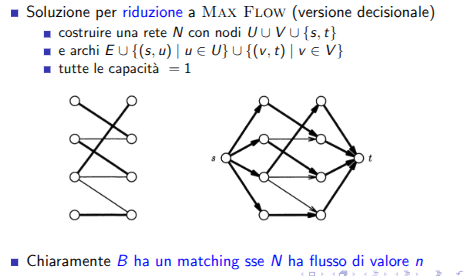
\includegraphics[width=\textwidth]{images/bipartite_matching.png}
\end{figure}


\subsection{Riduzione di $\HAMILTONPATH$ a $\SAT$}
\label{riduzione:hamiltonpath_sat}
Codifichiamo il problema in una formula di logica proposizionale in CNF (congiunzione di clausole, ogni clausola ha solo disgiunzioni).
Usiamo $|V|^2$ variabili booleane vere sse il vertice $v$ è nella $i$-esima posizione del cammino
\[x_{vi} \iff \pi(i) = v\]

Iniziamo a codificare $\pi$ come funzione biettiva. \\
Notiamo che, siccome dominio e codominio sono insiemi finiti e hanno la stessa cardinalitá, l'iniettivitá basta da sola a garantire anche la suriettivitá. \\
Inoltre, se $\pi$ é biettiva, allora é equivalente dire che ogni elemento del dominio é associato a un solo elemento del codominio, o viceversa. \\
Per chiarezza, anche se sono sufficienti le prime due, scriviamo comunque tutte e quattro le condizioni. \\

Nota: per semplificare la lettura possiamo immaginare $\bigwedge$ come $\forall$, e $\bigvee$ come $\exists$.
Non possiamo usare direttamente i quantificatori perché $\SAT$ é per la logica proposizionale 
(la soddisfacibilitá della logica del primo ordine é solo parzialmente calcolabile). \\ 

Inoltre, si puó usare De Morgan per convertire l'OR di negazioni (necessario per descrivere in CNF le clausole che impongono l'unicitá di qualcosa) nella negazione di un AND, che puó essere piú intuitiva.\\

\begin{enumerate}
    \item $\pi$ é una funzione: ogni posizione contiene almeno un vertice:\\
    \[\bigwedge_{i=1}^{|V|} \left( \bigvee_{v \in V} x_{vi} \right)\]
    \item $\pi$ é iniettiva: ogni posizione contiene un solo vertice:\\
    \[\bigwedge_{i=1}^{|V|} \left( \bigwedge_{v \in V} \bigwedge_{u \neq v} (\neg x_{vi} \lor \neg x_{ui}) \right)\] \\
\item $\pi$ é suriettiva: ogni vertice deve apparire nel ciclo almeno una volta:\\
    \[\bigwedge_{v \in V} \left( \bigvee_{i=1}^{|V|} x_{vi} \right)\]
    \item $\pi^{-1}$ é iniettiva: ogni vertice deve apparire nel ciclo una sola volta:\\
    \[\bigwedge_{v \in V} \left( \bigwedge_{i=1}^{|V|} \bigwedge_{j \neq i} (\neg x_{vi} \lor \neg x_{vj}) \right)\]
\end{enumerate}

Per codificare che vertici consecutivi nel cammino devono essere collegati da un arco:
\[
\bigwedge_{(u,v) \notin E} \left( \bigwedge_{i=1}^{|V|-1} (\neg x_{ui} \lor \neg x_{v(i+1)}) \land (\neg x_{u|V|} \lor \neg x_{v1}) \right)
\] \\

Sia $R$ la congiunzione di tutte queste formule. \\
Bisogna verificare la correttezza e l'efficienza della riduzione.
\subsubsection{Correttezza}
$R$ é soddisfacibile se e solo se esiste un cammino hamiltoniano in $G$.
\begin{proof}
Essendo una doppia implicazione, dobbiamo dimostrare entrambe le direzioni.

\textbf{1. $R$ é soddisfacibile $\implies$ esiste un cammino hamiltoniano in $G$.} \\
Se esiste un modello $M \models R$, allora:
\begin{itemize}
    \item per ogni vertice $v$, esattamente una variabile $x_{vi}$ é soddisfatta da $M$
    \item per ogni posizione $i$, esattamente una variabile $x_{vi}$ é soddisfatta da $M$
\end{itemize}
Ponendo $\pi(i) = v$ se e solo se $M \models x_{vi}$, otteniamo una permutazione dei vertici. \\

Inoltre, dall'ultima formula, abbiamo che $M \models \neg (x_{ui} \land x_{v(i+1)})$ per ogni coppia $(u,v) \notin E$, 
quindi $\pi(i)$ e $\pi(i+1)$ sono necessariamente collegati da un arco in $G$. \\
Stesso discorso per $\pi(|V|)$ e $\pi(1)$. \\

E queste sono esattamente le condizioni per avere un cammino hamiltoniano in $G$. \\

\textbf{2. Esiste un cammino hamiltoniano in $G$ $\implies$ $R$ é soddisfacibile.} \\
Dalla definizione di cammino hamiltoniano, sappiamo che esiste una permutazione dei vertici, in cui vertici consecutivi sono collegati da un arco. \\

L'ultima formula é resa vera dal fatto che vertici consecutivi sono collegati da un arco:
$(u, v) \notin E \implies \neg (x_{ui} \land x_{v(i+1)})$ \\

Le prime formule sono soddisfatte dal fatto che $\pi$ é una permutazione:
\begin{itemize}
    \item ogni vertice appare esattamente una volta, quindi esattamente una variabile $x_{vi}$ é vera per ogni vertice $v$
    \item ogni posizione contiene esattamente un vertice, quindi esattamente una variabile $x_{vi}$ é vera per ogni posizione $i$
\end{itemize}

E questo soddisfa la formula $R$. \\
\end{proof}

\subsubsection{Efficienza}
$R$ puó essere calcolata da una MdT deterministica in tempo polinomiale e spazio logaritmico.
\begin{proof}
La MdT funziona cosí:
\begin{enumerate}
    \item Scandisce l'input, conta i vertici e salva il numero $|V|$ in binario su un nastro.
    \item Usa tre contatori da $1$ a $|V|$ su tre nastri diversi per iterare su vertici e posizioni.
    \item Genera le prime quattro formule, iterando con i contatori e scrivendo le clausole sul nastro di output.
    \item Per l'ultima formula, itera con i contatori e genera di volta in volta la clausole $x_{ui} \lor x_{v(i+1)}$, sovrascrivendo quella precedente.\\
    Anche quelle che non dovrebbero esserci, cioé quelle per cui $(u,v) \in E$.
    \item Dopo ogni clausola generata, scandisce di nuovo l'input per verificare se $(u,v) \notin E$ e, in tal caso, 
    copia la clausola sul nastro di output. Poi passa all'iterazione successiva.
\end{enumerate}
I contatori occupano spazio $log(n)$. \\
Le clausole $x_{ui} \lor x_{v(i+1)}$ usano spazio per scrivere $(u, i, v, i+1)$. \\
I vertici sono codificati come numeri interi in binario, quindi $4 \cdot log(n) = O(log(n))$. \\
Lo spazio é logaritmico. \\

L'input viene scandito in tempo $O(n)$ dopo ogni clausola generata, e vengono generate $O(n^3)$ clausole. \\
Quindi il tempo é $O(n^4)$, cioé polinomiale. \\
\end{proof}